\chapter{Mathematical Theory of Tipping Points and Early Warning Signals}
\label{sec:intro2}
\graphicspath{{introduction2/figs}}

\lettrine[lines=3,loversize=0.1,findent=0.1em,nindent=0em]{H}{aving} explained, in \cref{sec:intro1}, the relevance of tipping elements to the Earth system, I will now review
the theory behind tipping points in this chapter. To do this I will categorise the ways in which a system can tip. I will also give an example of a system undergoing 
each of these types of tipping. In part due to the difficulties in accurately representing tipping points in Earth System Models (ESMs), it has become popular to
look for generic `early warning signals' of tipping points. I give a summary of these techniques and how they have been applied to Earth system tipping elements
at the end of the chapter.


\section{A Typology of Tipping Points}
\label{sec:tipping_typology}
It is helpful to classify tipping according to a typology developed by~\cite{Ashwin2012}. They identified three types of tipping:
\begin{description}
\item[B-tipping] which refers to a tipping caused by a system crossing a bifurcation due to a change in a parameter of the system.
\item[N-tipping] which refers to a tipping caused by noisy fluctuations driving the system  from one attractor to another.
\item[R-tipping] which  refers to a tipping caused by a system failing to track its continuously changing attractor. The `R' is for `rate' because the attractor is changing too
  fast for the system to adapt to it.
\end{description}

Since then, other researchers have found it useful to consider additional types of tipping. For example,~\cite{Halekotte2020} introduced the concept of shock or S-tipping which is
when a single large perturbation can push the system into a new state. When the system's attractor is not a steady state but is instead a limit cycle, the tipping can depend on the
phase of the cycle, a phenomenon which has been dubbed P-tipping \parencite{Alkhayuon2021}. More generally, if the tipping depends on the system's location on its attractor
then it is known as partial tipping \parencite{Alkhayuon2018}. In spatial systems, fragmented tipping is possible \parencite{Bastiaansen2022} in which only part of the domain
experiences tipping.

A more detailed examination of B,N,R and S tipping will now be given.

\subsection{B-Tipping}
\label{sec:btipping}
\subsubsection{Theory}
Consider a system with a state variable $\bm{x} \in \mathbb{R}^n$ described by the system of ordinary  differential equations
\begin{equation}
  \label{eq:generic_system}
  \dv{\bm{x}}{t} = \bm{f}(\bm{x}).
\end{equation}
Suppose the system has a fixed point at $\bm{x}^*$, such that $\bm{f}(\bm{x}^*)=0$ then the linear stability of the system \parencite{Strogatz2015} is characterised by
the behaviour of a small perturbation $\bm{y}$ about this fixed point, where $\bm{y} = \bm{x} - \bm{x}^*$. Then the dynamics of $\bm{y}$ are governed by
\begin{equation}
  \label{eq:linearised_equation}
  \dv{\bm{y}}{t} = J\bm{y} 
\end{equation}
where terms of order $\mathcal{O}\left(\left|\bm{y}\right|^2\right)$ or higher have been neglected and $J$ is a matrix called the Jacobian defined by
\begin{equation}
  \label{eq:jacobian}
  J_{ij} = \eval{\pdv{\bm{f}_i}{\bm{x}_j}}_{\bm{x}=\bm{x}^*}.
\end{equation}
The solution to \cref{eq:linearised_equation} is
\begin{equation}
  \label{eq:solution_to_linearised_equation}
  \bm{y} = e^{tJ}\bm{y}(0).
\end{equation}
Suppose $J$ has $n$ linearly independent eigenvectors (although similar conclusions will hold if it does not \parencite{guckenheimer2013}).
Let the set of eigenvectors be $\{\bm{v}_i\}$ and the set of eigenvalues $\{\lambda_i\}$ then \cref{eq:solution_to_linearised_equation} can be written as
\begin{equation}
  \label{eq:solution_to_linearised_equation_eigen}
  \bm{y} = \sum_i c_i e^{t\lambda_i}\bm{v}_i
\end{equation}
where $\{c_i\}$ are a set of constants chosen to match the initial conditions. It can be seen then that the long-time behaviour of $\bm{y}$ is
$\bm{y} \sim c_1 e^{t\lambda_1} \bm{v}_1$ where $\lambda_1$ is the eigenvalue with largest real part. If this is positive, then $\bm{y}$ will leave the vicinity of $\bm{x}^*$, whereas
if it is negative $\bm{y}$ will approach $\bm{x}^*$. Suppose $\bm{x}^*$ is a hyperbolic fixed point, which means that $J$ has no eigenvalues with zero real part. Then the Hartman-Grobman Theorem
\parencite{Grobman1959,Hartman1960,Hartman1963} guarantees that the trajectories of $\bm{y}$ will be topologically conjugate --- that is to say qualitatively the same --- in some
neighbourhood of $\bm{x}^*$ to the trajectories of $\bm{x}$.  This means that $\bm{x}^*$ is linearly stable only when $J$ has eigenvalues with only negative real parts.
The directions $\bm{v}_k$ with $\Re \lambda_k < 0$ are known as stable directions (as the flow is attracted to the fixed point along these directions),
those with $\Re \lambda_k > 0$ are unstable directions \parencite{Strogatz2015}.

B- or Bifurcation-tipping refers to tipping which is driven by changes to the stability, or the loss altogether, of these fixed points.
A bifurcation is a concept from the mathematical theory of dynamical systems, introduced by~\cite{Poincare1885}.
It is used to describe a situation where the fixed points of a system qualitatively change as a control parameter is varied.

Consider a modification to \cref{eq:generic_system} where a control parameter $\mu \in \mathbb{R}$ (which could, for example, be atmospheric \ce{CO2}) has been introduced
\begin{equation}
  \label{eq:generic_system_control_parameter}
  \dv{\bm{x}}{t} = \bm{f}_{\mu}(\bm{x}).
\end{equation}
The fixed points are described by $\bm{f}_{\mu}(\bm{x}^*) = 0$. By the Implicit Function Theorem \parencite{Spivak1965}, $\bm{x}^*$ is a smooth
function of $\mu$ except at points where $J$ has a zero eigenvalue, these points in $(\bm{x},\mu)$ space are known as bifurcation points.
Other bifurcation points can occur when a stable fixed point becomes unstable (or vice versa). In both cases an eigenvalue of $J$ must cross the imaginary
axis, i.e.\ have zero real part \parencite{guckenheimer2013}. As a result of this, the Hartman-Grobman Theorem is not applicable and so a non-linear analysis must be undertaken.

Fortunately, there are techniques to deal with this, using the Centre Manifold Theorem \parencite{Morris1977}, which can be stated loosely as
\begin{theorem}[Centre Manifold Theorem]
  \label{thm:centre_manifold_theorem}
  Let the eigenvalues, $\{\lambda_i\}$, of $J$ be divided into three sets such that $\spec J = \sigma_s \cup \sigma_u \cup \sigma_c$, where $\sigma_s = \{\lambda_i : \Re \lambda_i < 0\}$,
  $\sigma_u = \{\lambda_i : \Re \lambda_i > 0\}$ and $\sigma_c = \{\lambda_i : \Re \lambda_i = 0\}$.
  Let their respective eigenspaces be $E_s$, $E_u$ and $E_c$. Then there are stable and unstable invariant manifolds $W_s$  and $W_u$ tangent to $E_s$ and  $E_u$ at $\bm{x}^{*}$,
  and a centre manifold $W_c$ tangent to $E_c$ at $\bm{x}^*$.
\end{theorem}
The upshot of this theorem is that the dynamics are now controlled by the centre manifold. Suppose that the unstable manifold is empty (the most relevant case for tipping point research)
then \cref{thm:centre_manifold_theorem} implies that the dynamics are topologically conjugate to
\begin{subequations}
  \label{eq:centre_manifold_topological_equivalence}
  \begin{align}
  \dv{\bm{u}}{t} &= g(\bm{u}) \\
  \dv{\bm{v}}{t} &= -\bm{v}
  \end{align}
\end{subequations}
with $(\bm{u},\bm{v}) \in W_c \times W_s$. At long times $\bm{v} \rightarrow \bm{0}$ so at long times the dynamics are given by $\bm{u}$ on the centre manifold
\parencite{guckenheimer2013}. In order to calculate $g$, suppose that
$\bm{x} = (\bm{u},\bm{z}) \in \mathbb{R}^n$ so that
\begin{subequations}
  \label{eq:block_diagonal}
  \begin{align}
    \dv{\bm{u}}{t} &= A\bm{u} + p(\bm{u},\bm{z}) \\
    \dv{\bm{z}}{t} &= B\bm{z} + q(\bm{u},\bm{z})
  \end{align}
\end{subequations}
where $A,B$ have eigenvalues with zero and negative real parts respectively and $p,q$ are nonlinear functions without any linear terms.
Then the centre manifold can be written as a graph $W_c = (\bm{u},h(\bm{u}))$
with $\bm{z} = h(\bm{u})$, so that on the centre manifold
\begin{equation}
  \label{eq:dynamics_on_the_centre_manifold}
  \dv{\bm{u}}{t} = A\bm{u} + p\left(\bm{u},h\left(\bm{u}\right)\right).
\end{equation}
The next step is to make \cref{eq:dynamics_on_the_centre_manifold} as simple as possible. By the Hartman-Grobman Theorem, \cref{eq:dynamics_on_the_centre_manifold}
cannot be linearised. However the next most simplest approach is to use normal forms, which describe the different sorts of possible bifurcations \parencite{Dijkstra2011}.

Consider again \cref{eq:generic_system_control_parameter}, but now enlarge the state space to $\mathbb{R}^{n+1}$ by viewing $\mu$ as a dynamic variable with $\dot{\mu} = 0$. Suppose
further, without loss of generality, that there is a bifurcation point at $(\bm{x},\mu)  = (\bm{0},0)$ where $J$ has a simple zero eigenvalue.
Then using \cref{thm:centre_manifold_theorem} a centre manifold passing through
$(\bm{0},0)$ can be found. If the trajectories are restricted to the centre manifold and certain transversality conditions are met ($\partial_{\mu}f \neq 0,\partial_{xx} f\neq 0$ at the
bifurcation point) the trajectories will be topologically equivalent \parencite{guckenheimer2013} to
\begin{equation}
  \label{eq:saddle_node}
  \dv{x}{t}  = \mu + x^2.
\end{equation}
This type of bifurcation is known as a saddle-node or a fold bifurcation.
This remarkable fact has simplified a high dimensional dynamical system to a generic one-dimensional system near the bifurcation point \parencite{Glendinning1994}.

The saddle-node bifurcation is very important as other bifurcation problems can be perturbed into a saddle-node bifurcation problem (as it is unusual for the transversality conditions
not to be met). In this sense, saddle-nodes are the type of bifurcations to be expected in nature. However if the transversality conditions are not met other types of bifurcations can arise.

If $\partial_{\mu}f=0$, then the system is equivalent to
\begin{equation}
  \label{eq:transcritical}
  \dv{x}{t} = \mu x - x^2,
\end{equation}
which is the normal form for a transcritical bifurcation. If $\partial_{\mu}f = 0$ and $\partial_{xx}f=0$ with $\partial_{xxx}f \neq 0$
the bifurcation is known as a pitchfork bifurcation with normal form
\begin{equation}
  \label{eq:pitchfork}
  \dv{x}{t} = \mu x - x^3.
\end{equation}

Another important sort of bifurcation is a Hopf bifurcation \parencite{Hopf1942}. For this bifurcation, a complex conjugate eigenvalue pair become purely imaginary, $\lambda = \pm i\omega$.
As there are no zero eigenvalues the Implicit Function Theorem implies no new equilibria will be created. However it will lead to a change in the dimensions of the
stable and unstable manifolds, leading to a qualitative change in the behaviour of the system. It can be shown that there is a centre manifold on which a limit cycle can exist
\parencite{guckenheimer2013}. In other words, these bifurcations lead to the creation of periodic oscillatory behaviour. These bifurcations
can occur only in systems of dimension two or higher. The normal form of this bifurcation \parencite{Kuznetsov2004} can be expressed as a differential equation involving the complex variable $z = x + iy$
\begin{equation}
  \label{eq:hopf}
  \dv{z}{t} = (\mu + i) z - z|z|^2.
\end{equation}

\subsubsection{Stommel's AMOC Model}
As an example of B-tipping, consider Stommel's AMOC model \parencite{STOMMEL1961}, which after a rescaling \parencite{Dijkstra2011} can be written as:
\begin{subequations}
  \label{eq:stommel_amoc}
  \begin{align}
    \dv{T}{t} &= \eta_1 - T\left(1 - \left|\Psi\right|\right) \\
    \dv{S}{t} &= \eta_2 - S\left(\eta_3 + \left|\Psi\right|\right) \\
    \Psi      &= T - S
  \end{align}
\end{subequations}
where $T$ and $S$ are (dimensionless) equator to pole temperature and salinity differences respectively.
The flux $\Psi = T - S$ is the strength of the AMOC\@. The parameters $\eta_1,\eta_2,\eta_3$ represent
thermal forcing, freshwater forcing and the ratio of their timescales respectively.

\Cref{fig:stommel_amoc} shows the equilibria of \cref{eq:stommel_amoc} as well the solution to \cref{eq:stommel_amoc} for the case where $\eta_2$ slowly increases to a maximum and then slowly
decreases again following a parabolic trajectory.
As $\eta_2$ is increased the strength of the AMOC decreases until it reaches a saddle-node bifurcation point
at $\eta_2^*  \approx 1.2$ where the AMOC abruptly transitions to a weaker state with flow in the opposite direction.
Near the bifurcation point, the flux behaves like $\Psi \sim \sqrt{\eta_2^*-\eta_2}$,
which reflects the normal form \cref{eq:saddle_node}. Note that when $\eta_2$ is decreased, it must be brought down to the lower value of $0.9$ to transition back into its original state.
This is known as hysteresis.


\begin{figure}
  \centering
  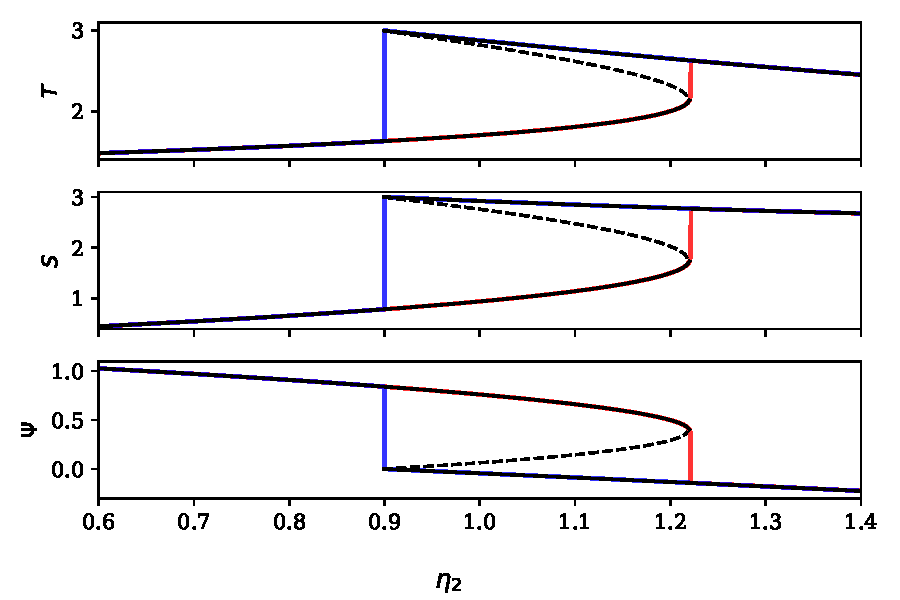
\includegraphics[width=\textwidth,keepaspectratio]{stommel}
  \caption[The Stommel Model of the AMOC]{This shows the state of the Stommel model, \cref{eq:stommel_amoc}, as a function of the parameter $\eta_2$. 
    The stable equilibrium states are given by solid black lines and the unstable states are given by the black dashed line.
    The red line shows the instantaneous state of the AMOC for $\eta_2$ slowly increasing from $0.6$ to $1.4$. The blue line
    shows the instantaneous state for $\eta_2$ decreasing from $1.4$ to $0.6$.
    As $\eta_2$ is increased, the AMOC transitions from a strong poleward flow to a weaker equatorward state. Note that near the
    bifurcation point around $\eta_2 \approx 1.2$ the stable states seem to behave like the square root of the control parameter. This reflects the normal form of
    the bifurcation. Note that when $\eta_2$ is decreased the transition back to the poleward flow state happens at a lower value
    of $\eta_2$ --- this is an example of hysteresis. The other parameters were set to $\eta_1 = 3,\eta_3=0.3$.}
  \label{fig:stommel_amoc}
\end{figure}
\subsection{N-tipping}
If a system with multiple stable states is subject to stochastic forcing, then it will perform transitions between these states if observed for long enough. This
phenomenon is called N- or noise-tipping. This has an important difference to B-tipping. In B-tipping an external driver changes a control parameter, causing a system to tip
but in N-tipping the natural variability of the system causes it to tip.

The role of noise in the climate system was identified by~\cite{Hasselmann1976}. He viewed the `slow' components of the Earth system (the ocean, the vegetation and the ice sheets) as being
deterministic and the `fast' components (the atmosphere) as being essentially stochastic. This stochasticity may be viewed as an effective model for chaotic systems \parencite{Lorenz1963}
or resulting from unresolved processes \parencite{Palmer2009}. Certain paleoclimate abrupt shifts, such as the Dansgaard-Oeschger events, have been viewed as N-tipping \parencite{Ditlevsen1999}.

Stochastic differential equations can be written \parencite{Jacobs2010} as
\begin{equation}
  \label{eq:general_sde}
  \dv{\bm{x}}{t} = \bm{F}(\bm{x}) + G(\bm{x})\bm{\eta}(t).
\end{equation}
The vector function $\bm{F}$ represents the deterministic evolution and the matrix function $G$ represents the stochastic evolution. The function
$\bm{\eta}(t) = \dv*{\bm{W}}{t}$ is known as white noise and is the derivative of a Wiener process. It is the source of the stochasticity.
It has mean zero and is `delta correlated' in time, by which is meant
\begin{equation}
  \label{eq:eta_correlation}
  \E\left(\bm{\eta}_i(t)\bm{\eta}_j(t')\right) = \delta_{ij}\delta(t-t')
\end{equation}
where $\delta_{ij}$ is the Kronecker delta and $\delta(t-t')$ is the Dirac delta function. This notation is somewhat misleading as it suggests that all the functions involved are
differentiable, however realisations of the Wiener process are almost surely not differentiable \parencite{Mckean2014}. More rigorously, \cref{eq:general_sde} should be written as
\begin{equation}
  \label{eq:general_sde_maths}
  \dd{\bm{x}_t} = \bm{F}(\bm{x}_t)\dd{t} + G(\bm{x}_t)\dd{\bm{W}_t}
\end{equation}
where the differentials are understood to imply integration. The notation of \cref{eq:general_sde} tends to be favoured by physicists and that of \cref{eq:general_sde_maths} by
mathematicians.

Viewing individual solutions of \cref{eq:general_sde}, or sample paths, is one approach  to analysing stochastic systems. Another useful approach is to calculate the probability density function
(pdf), $p(\bm{x},t)$ of $\bm{x}$ and how it evolves in time. The tool to do this is the Fokker-Planck equation \parencite{Fokker1914,Planck1917}, given by
\begin{equation}
  \label{eq:fokker_planck}
  \pdv{p}{t} = - \sum_i \partial_i \left(\bm{F}_i p\right) + \sum_i\sum_j \partial_i\partial_j \left(D_{ij} p\right)
\end{equation}
where $D = GG^T/2$.

\subsubsection{Kramers' Escape Rate}
Often a very simple one-dimensional model is used in studies of N-tipping
\begin{equation}
  \label{eq:simple_sde}
  \dv{x}{t} = -\dv{U}{x} + \sigma \eta(t).
\end{equation}
This is an example of a potential system because the deterministic dynamics are given by the gradient of a potential function, $U(x)$. Any one dimensional system can be put in this form
but that is not always the case for higher dimensional systems.
Furthermore, the noise is assumed to be `white', with constant variance $\sigma^2$. It is known as white noise because in the frequency domain, all
frequencies are excited with equal amplitude. This is a questionable assumption for the Earth system, where the spectrum is not white \parencite{Mitchell1976,VonderHeydt2021} and may
change due to climate change \parencite{Huntingford2013}.

\Cref{eq:simple_sde} has an associated Fokker-Planck equation
\begin{equation}
  \label{eq:fokker_planck_one_d}
  \pdv{p}{t} = \pdv{x} \left(\dv{U}{x}p\right) + \frac{1}{2}\sigma^2 \pdv[2]{p}{x},
\end{equation}
which can also be written in the form of a continuity equation
\begin{equation}
  \label{eq:fokker_planck_continuity}
  \pdv{p}{t} + \pdv{J}{x} = 0
\end{equation}
where $J$ is the probability current given by
\begin{equation}
  \label{eq:probability_current}
  J(x) = -\dv{U}{x}p - \frac{1}{2}\sigma^2 \pdv{p}{x}.
\end{equation}

If \cref{eq:simple_sde} has multiple stable states, then an estimate of the transition rate between these states can be made. This estimate is known
as the Kramers' Rate \parencite{Kramers1940}. This derivation follows~\cite{Risken1984}.

\begin{figure}
  \centering
  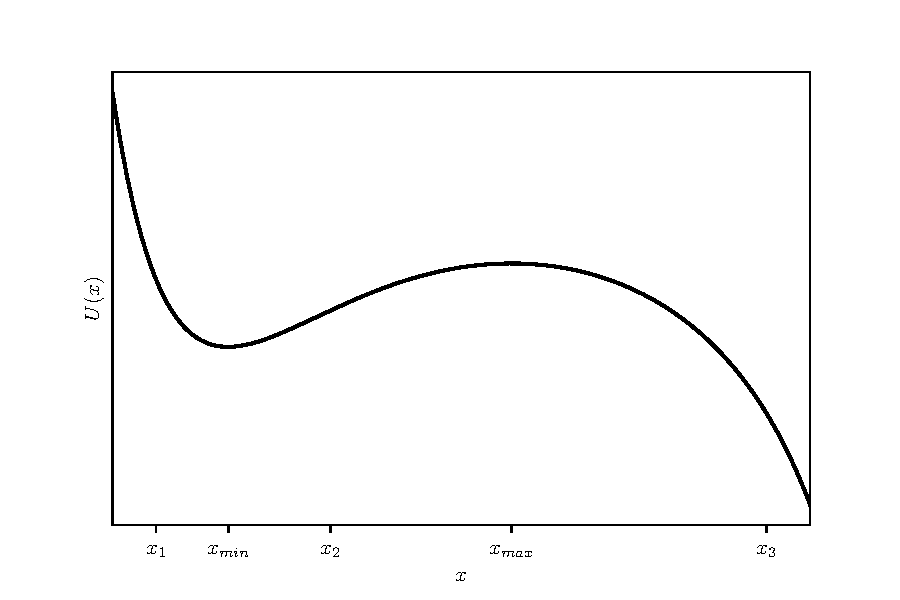
\includegraphics[width=\textwidth,keepaspectratio]{potential_to_escape}
  \caption[Escape from potential well]{An example of a potential with a stable state at $x_{min}$ from which a system can escape over the potential barrier at
    $x_{max}$ to a new state near $x_3$. The precise locations of $x_1,x_2,x_3$ do not matter at the level of approximation Kramers' escape rate formula works at.}
  \label{fig:potential_to_escape}
\end{figure}

Suppose that $U$ has the form given by \cref{fig:potential_to_escape}, which has a stable state at $x_{min}$, an unstable state at $x_{max}$. The rate at which the system
transitions from near $x_{min}$, in the region between $x_1$ and $x_2$, to the other side of the maximum, near $x_3$, is to be determined.
Assuming the system is in a near steady state, \cref{eq:fokker_planck_continuity}
implies that $J$ is approximately constant. By multiplying \cref{eq:probability_current} by the integrating factor $\exp \frac{2U(x)}{\sigma^2}$, $J$ can be put into the form
\begin{equation}
  \label{eq:probability_current_other_form}
  J = -\frac{1}{2}\sigma^2 e^{-\frac{2U(x)}{\sigma^2}} \pdv{x} \left( p(x) e^{\frac{2U(x)}{\sigma^2}}\right).
\end{equation}
This can then be integrated from $x_{min}$ to $x_3$ give
\begin{equation}
  \label{eq:integrated_J}
  J = \frac{\sigma^2}{2} \left(p(x_{min})e^{\frac{2U(x_{min})}{\sigma^2}} - p(x_3)e^{\frac{2U(x_{3})}{\sigma^2}}\right)\left(\int_{x_{min}}^{x_{3}} e^{\frac{2U(x)}{\sigma^2}} \dd{x}\right)^{-1}.
\end{equation}
As it will be rare to find the system at $x_3$, as the noise is weak enough to make the transitions rare, $p(x_3)$ is negligible.
To estimate $p(x_{min})$, assume this is given by the equilibrium distribution which can be found by setting $J$ to
a constant. This constant can be chosen to be the value of $J$ at $x_{min}$, giving the following expression for the equilibrium pdf, $p_{eq}$,
\begin{equation}
  \label{eq:equilibrium_pdf}
  p_{eq}(x) = p(x_{min})e^{\frac{2U(x_{min})}{\sigma^2}}e^{-\frac{2U(x)}{\sigma^2}}.
\end{equation}
The probability of finding the system near $x_{min}$ is therefore
\begin{equation}
  \label{eq:p_near_xmin}
  P = \int_{x_1}^{x_2} p_{eq}(x) \dd{x} = p(x_{min})e^{\frac{2U(x_{min})}{\sigma^2}} \int_{x_1}^{x_2} e^{-\frac{2U(x)}{\sigma^2}} \dd{x}.
\end{equation}
The escape rate is $r = J/P$ which becomes
\begin{equation}
  \label{eq:escape_rate_integrals}
  r^{-1} = \frac{2}{\sigma^2} \int_{x_1}^{x_2} e^{-\frac{2U(x)}{\sigma^2}} \dd{x} \int_{x_{min}}^{x_3} e^{-\frac{2U(x)}{\sigma^2}} \dd{x}.
\end{equation}
Each integral can be asymptotically evaluated using Laplace's Method \parencite{Bender1978} to give Kramers' escape rate
\begin{equation}
  \label{eq:kramers}
  r^{-1} \sim \frac{2\pi}{\sqrt{U''(x_{min})|U''(x_{max})|}} e^{\frac{2}{\sigma^2}\left(U(x_{max})-U(x_{min})\right)},
\end{equation}
for $ \sigma \rightarrow 0$.

\subsubsection{Example}
As an example consider the potential
\begin{equation}
  \label{eq:example_potential}
  U(x) = -\frac{1}{2}x^2 + \frac{1}{12}x^4
\end{equation}
which has symmetric stable states at $x = \pm \sqrt{3}$. There is a potential barrier at $x = 0$. Assuming that $\sigma = 0.75$, Kramers' rate predicts a transition
timescale of $r^{-1} \approx 65$ time units. \Cref{fig:ntipping} shows transitions happening on this timescale.

\begin{figure}
  \centering
  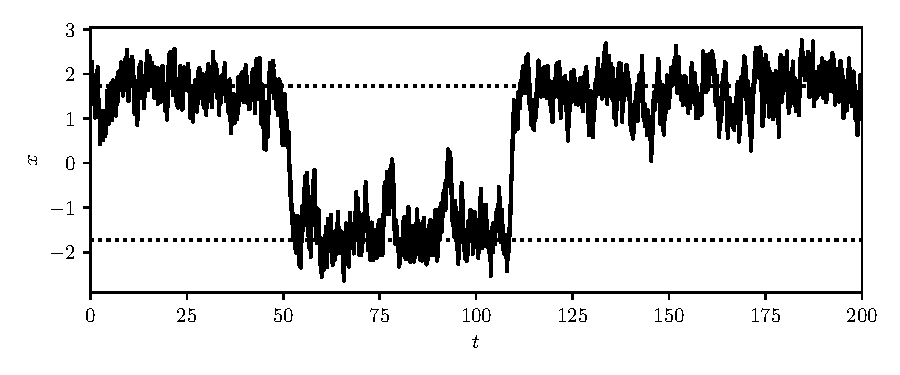
\includegraphics[width=\textwidth,keepaspectratio]{noise_trans}
  \caption[An example of N-tipping]{A time series showing transitions between two stable states (indicated by a dotted line). Kramers' formula, \cref{eq:kramers} predicts a
    transition timescale of about $65$ time units. The time series shows transitions happening on this timescale.}
  \label{fig:ntipping}
\end{figure}


\subsection{R-tipping}
A relatively recently discovered type of tipping is R-tipping. First discovered by~\cite{Luke2011} in a simple model of soil temperatures, R-tipping or rate-induced tipping refers to
a situation where the rate of change of a control parameter, rather than the magnitude of the parameter itself  controls whether a system tips or not \parencite{Wieczorek2011}.
This type of tipping occurs in nonautonomous dynamical systems, which is a system with explicit time dependence \parencite{Ashwin2017a}.

This sort of tipping is best explained through an example, taken from~\cite{Ashwin2012}. The system is
\begin{subequations}
  \label{eq:rtipping_example}
  \begin{align}
    \dv{x}{t}   &= \left(x + \mu\right)^2 - 4 \label{eq:rtipping_example_x} \\
    \dv{\mu}{t} &= r.                          \label{eq:rtipping_example_r} 
  \end{align}
\end{subequations}
These equations can be interpreted as a system with state $x$ in a changing environment represented by parameter $\mu$ that changes at some finite rate, $r$.

\begin{figure}
  \centering
  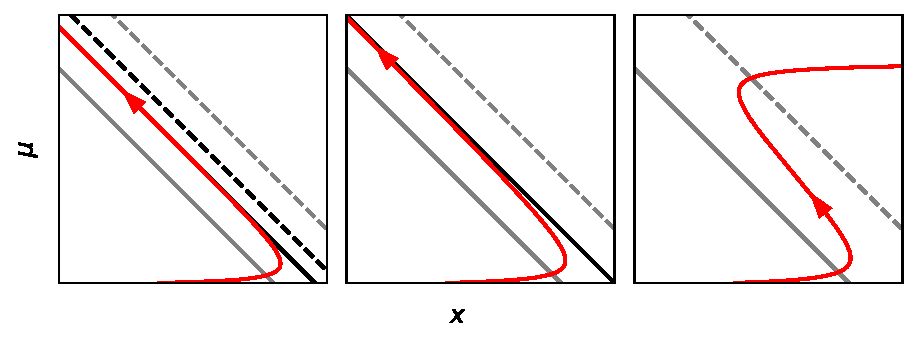
\includegraphics[width=\textwidth,keepaspectratio]{rate}
  \caption[R-tipping mechanism]{Panels showing the state space of a system, \cref{eq:rtipping_example}, undergoing R-tipping.
    From left to right, the figures show the system below the critical rate, at the critical rate and above the critical rate. In the left panel, with $r=3.2$ the lines
    $x^{\mathrm{PB}}_{\pm}$ exist and are separated. In the centre panel with $r = r_c = 4$, $x^{\mathrm{PB}}_{\pm}$ exist and have collided into one line. In the right panel,
    $r = 4.8$ and therefore $x^{\mathrm{PB}}_{\pm}$ do not exist. As a result trajectories diverge as the system has undergone R-tipping. Note that for all values of $r$, the
    quasi-static equilibria exist.}
  \label{fig:rate_tipping}
\end{figure}

Consider the `frozen system' \parencite{Wieczorek2021}, which is \cref{eq:rtipping_example_x} with $\mu$ constant --- this describes the dynamics
in the case where the environment is unchanging. It has equilibria at
$x^*_{\pm} = \pm 2 - \mu$. The stability of these equilibria can be found in the manner described in \cref{sec:btipping}, which in this case amounts to evaluating
the derivative of \cref{eq:rtipping_example_x} with respect to $x$ at $x^*_{\pm}$. These quasi-static equilibria are shown as grey lines in \cref{fig:rate_tipping}, where
the stable quasi-static equilibria are shown in solid grey and the unstable quasi-static equilibria are shown as a dashed line.
It can be shown that $x_-$ is stable for all $\mu$ values, and $x_+$ is unstable for all $\mu$ values. As a result a na{\"\i}ve B-tipping analysis
would suggest this system cannot tip. However, as will be shown, this system can undergo R-tipping.

To see this, make a change of coordinates into a co-moving frame by setting $y = x + \mu$. Then the system becomes
\begin{equation}
  \label{eq:rtipping_co_moving}
  \dv{y}{t} = y^2 + r - 4.
\end{equation}
This equation has a stable fixed point at $-\sqrt{4-r}$ and an unstable fixed point at $\sqrt{4-r}$. Returning to the $x$ coordinates these solutions correspond to the
pullback attractor and repeller of the system, $x^{\mathrm{PB}}_{\pm} = \pm \sqrt{4 - r} - \mu$. These pullback objects are the appropriate generalisation of attractors and repellers to the
nonautonomous case \parencite{Ghil2020a}. They are plotted in black in \cref{fig:rate_tipping} where the solid line
is the stable state and the dashed line is unstable. It is to $x_-^{\mathrm{PB}}$ rather than $x_-$ that the solutions of \cref{eq:rtipping_example} are attracted to, plotted in red
in \cref{fig:rate_tipping}.

If $r < 4$, then $x_-^{\mathrm{PB}}$ exists and so solutions evolve towards it. However if $r > 4$ then $x_-^{\mathrm{PB}}$ does not exist and so solutions diverge to infinity. As a result there
is a critical rate, $r_c = 4$, above which R-tipping occurs.

\subsubsection{The Compost Bomb}
The paradigmatic example of R-tipping is the Compost Bomb instability \parencite{Luke2011,Wieczorek2011,Clarke2021,OSullivan2023}, which is a thermal
instability in the soil. This phenomenon is caused by microbial respiration warming the soil, which in turn increases the soil temperature. However, this respiration decreases the supply
of soil carbon and thus decreases the amount of respiration and thus heating in the soil. Due to the differences between the (rapid) timescale of heating and the (slow) timescale of soil
carbon decrease there is the possibility for a dramatic increase in soil temperature.~\cite{Luke2011} found that if the air temperature raised faster than a critical rate then the
compost bomb instability would be caused. Their model was 
\begin{subequations}
  \label{eq:compost_bomb}
  \begin{align}
    \mu\dv{T_s}{t} &= -\lambda \left(T_s - T_a\right) + Ar_0 C_s e^{\alpha T_s} \\
    \dv{C_s}{t}    &= \Pi - r_0 C_s e^{\alpha T_s} \\
    \dv{T_a}{t}    &= v
  \end{align}
\end{subequations}
where $T_s$ is the soil temperature, $T_a$ is the air temperature and $C_s$ is the soil carbon. The parameters, taken from~\cite{Wieczorek2011}, are a heat capacity
$\mu = \SI{2.5E6}{\joule\per\meter\squared\per\kelvin}$, a thermal coupling $\lambda = \SI{5.049E6}{\joule\per\year\per\meter\squared\per\kelvin}$, a heat of
respiration $A = \SI{3.9E7}{\joule\per\kilo\gram\carbon}$, a specific respiration $r_0 = \SI{0.01}{\per\year}$, a temperature dependence of respiration $\alpha = \SI{0.09}{\per\kelvin}$
and a net primary productivity $\Pi = \SI{1.055}{\kilo\gram\carbon\per\meter\squared\per\year}$. When the rate of increase in temperature is increased above a critical rate,
$v \approx \SI{0.08}{\kelvin\per\year}$ the instability is triggered.

\begin{figure}
  \centering
  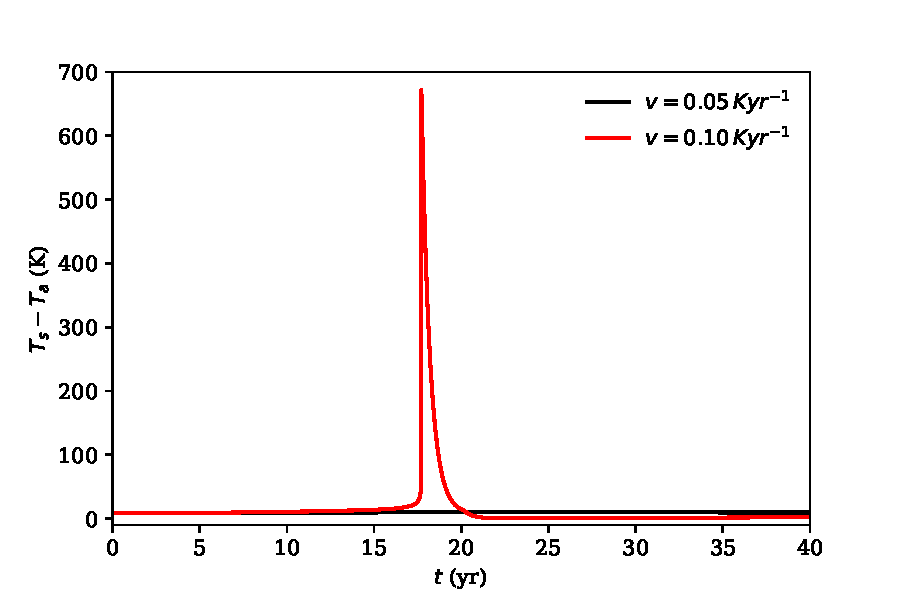
\includegraphics[width=\textwidth,keepaspectratio]{cbomb}
  \caption[Compost Bomb]{A plot of soil temperature relative to air temperature with two different rates of warming, calculated from \cref{eq:compost_bomb}. Note the spike in temperatures
  for high enough rates of warming---an example of R-tipping.}
  \label{fig:compost_bomb_example}
\end{figure}

\Cref{fig:compost_bomb_example} shows two time series of \cref{eq:compost_bomb} with $v = \SI{0.05}{\kelvin\per\year}$ and $v = \SI{0.1}{\kelvin\per\year}$. For the larger
rate of warming there is a clear spike in the soil temperatures.

\subsection{S-tipping}
A more recent addition to the tipping points typology is that of S- or shock-tipping. This refers to a situation where a single large perturbation
can push a system from one state to another \parencite{Halekotte2020,Feudel2023}, such as an extreme weather event on an ecosystem.
In this sense it is closely related to ideas of resilience introduced by~\cite{Holling1973}.

It is related to N-tipping but should be differentiated from it in the following sense. If $\bm{x}^*$ is a fixed point, with a basin of attraction $\mathcal{B}$ then the
smallest perturbation required to push the system into a new state is given by
\begin{equation}
  \label{eq:smallest_perturbation}
  \bm{\Delta} = \argmin \{ |\bm{x}'| : \bm{x}^* + \bm{x}' \notin \mathcal{B}\}.
\end{equation}
If the system is the potential system \cref{eq:simple_sde}, then this is equal in magnitude to the distance to the nearest maximum, $|x_{max} - x_{min}|$. This should be compared to Kramers' formula,
\cref{eq:kramers}, which is a function of the difference in potential $U(x_{max}) - U(x_{min})$. In other words, S-tipping depends on the distance to the potential barrier, but N-tipping depends on
the height of that barrier.

\subsubsection{Allee Effect}
Consider a population growing via logistic growth with carrying capacity $k$ that is subject to the Allee Effect \parencite{Allee1932,Stephens1999}, which is an effect that reduces
growth rates at low population densities. A simple model of this is
\begin{equation}
  \label{eq:allee_effect}
  \dv{x}{t} = x\left(x-1\right)\left(1-\frac{x}{k}\right),
\end{equation}
where $k > 1$ and $x$ is a population density. This has equilibria at $x_1 = 0$, $x_2 = 1$ and $x_3 = k$. The equilibria at $x_1$ and $x_3$ are stable. $x_1$ corresponds to an extinct
state and $x_3$ to a populated state.

If the system is initially in equilibrium at $x_3$, the distance to the basin boundary is $\Delta = |x_3 - x_2| = k - 1$. Hence if the system receives a kick of
this magnitude or greater then the system will transition to the extinction state. \Cref{fig:shock_tipping}, shows the evolution of $x$ as \cref{eq:allee_effect} is integrated
with $k = 2.0$ and given perturbations of magnitude $0.99$ and $1.01$ at times $25.0$ and $50.0$.
The first perturbation is not large enough to push the system across the boundary of the basin of attraction, yet the second one is,
which is why the population undergoes S-tipping after the second perturbation.

\begin{figure}
  \centering
  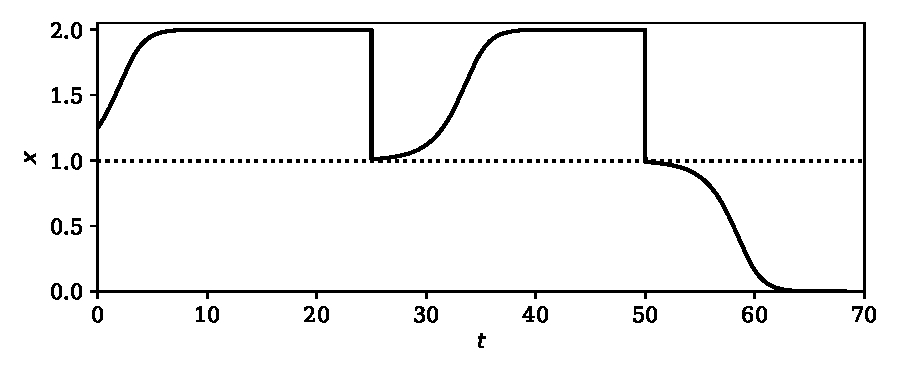
\includegraphics[width=\textwidth,keepaspectratio]{shock}
  \caption[Shock Tipping]{An example of shock-tipping. The system given by \cref{eq:allee_effect} receives a perturbation of $0.99$ at time $25.0$. This is not large enough to make it cross the basin boundary
    (given by the dotted line) and so the system recovers. However at time $50.0$ a perturbation of $1.01$ is given which is enough to make it cross the basin boundary and thus to make the
  population go extinct.}
  \label{fig:shock_tipping}
\end{figure}

\subsection{Tipping in Reality}
This typology has given the impression that individual tipping phenomena can be easily assigned to the categories of B,N,R or S-tipping. However this is not the case as any
real tipping point will have aspects of many of the different tipping types. For example, if a control parameter is changing such that the system is approaching a B-tipping point,
then Kramers' formula \cref{eq:kramers} implies that the system is more likely to undergo N-tipping. Furthermore, a system nearing a tipping point will be more likely to undergo S-tipping as
$\Delta$, defined by \cref{eq:smallest_perturbation}, is smaller as the basin of attraction shrinks. If a system is experiencing a shock, it is also likely that its parameters will
be changing quickly as well so this tipping will have an R-tipping character too.

Although real tipping points may have multiple characteristics it is still often possible and, more importantly, still useful to categorise the tipping into one of the above categories.


\section{Early Warning Signals}
Given the large impact a climate tipping point would have \parencite{Lenton2019a}, it would be useful to know at what level of climate forcing they would be triggered.
However models show little agreement about the level of forcing required to cause them \parencite{Drijfhout2015}. The processes of interest are by their nature
nonlinear and often involve interactions between the physical climate and the biosphere, where the `correct' equations are inherently uncertain. Furthermore,
some tipping behaviour may depend on subgrid scale processes, such as in the case of fire \parencite{Mangeon2016}. As a result a precise determination of the dangerous level of climate
forcing is challenging.

Instead, a theory of \emph{early warning signals} (EWS), sometimes known as  \emph{early warning indicators} (EWI), has emerged \parencite{Dakos2008,Scheffer2009,Lenton2011,Williamson2015}.
These techniques attempt to use certain generic statistical features of tipping points to provide an indication as to whether a system is
moving towards a tipping point. This is closely related to ideas about normal forms developed in \cref{sec:btipping}.

However not all types of tipping will give good early warning signals. Noise and shock tipping are not driven by a continuously changing external factor and
so early warning signals (in the conventional sense) will not be useful in these cases. For the case of rate tipping, there has been some work on
early warning signals \parencite{Ritchie2016}. However most of the work has been done
for bifurcation tipping where statistics can be calculated as a function of a slowly evolving parameter.

\subsection{Critical Slowing Down}
The basic idea of early warning signals is that of \emph{critical slowing down} \parencite{Dakos2008}. Suppose there is a system
\begin{equation}
  \label{eq:system}
  \dv{x}{t} = f(x,\mu)
\end{equation}
which has a stable state for $\mu < \mu_c$ at $x^*$ and undergoes a bifurcation when $\mu=\mu_c$. Then before the bifurcation, the system can be linearised about this steady state
to give
\begin{equation}
  \label{eq:linearised_about_steady_state}
  \dv{y}{t} = -\lambda y
\end{equation}
where $y = x -x^*$ and $\lambda = -f'(x^*,\mu)$. As the bifurcation is approached, $\lambda \rightarrow 0$ so any method that detects changes in $\lambda$ can act as an early warning
signal, in a quite generic way, for B-tipping.

Solving \cref{eq:linearised_about_steady_state} gives
\begin{equation}
  \label{eq:solved_linaer}
  y = e^{\lambda t} y(0)
\end{equation}
and so $\lambda^{-1}$ gives the timescale for perturbations to relax to equilibrium. This means that as $\lambda \rightarrow 0$,
this timescale approaches infinity, hence the name critical slowing down.


\subsection{Variance and Autocorrelation}
A very common way to approach early warning signals is to assume that the system of interest can be modelled as a one dimensional system subject to additive Gaussian white noise. The first
of these assumptions is defensible on the grounds that near a bifurcation point, generic systems behave qualitatively like \cref{eq:saddle_node}. The second assumption is more suspect
as systems are generally subject to time correlated noise, such as red noise. However in the case of red noise, as long as the dynamics are considered over long enough timescales, then the
noise can be approximated as white. This assumption amounts to analysing the Langevin equation \parencite{Langevin1908}
\begin{equation}
  \label{eq:stochastic_system}
  \dv{x}{t} = f(x) + \sigma \eta(t) 
\end{equation}
where $\eta$ is delta correlated noise and $\sigma^2$ is the variance of the noise. This system can then be linearised to give
\begin{equation}
  \label{eq:ou_process}
  \dv{y}{t} = -\lambda y + \sigma \eta(t)
\end{equation}
where $y$ and $\lambda$ are defined as in \cref{eq:linearised_about_steady_state}. This is the equation that defines an Ornstein-Uhlenbeck process \parencite{Uhlenbeck1930} and its statistical
properties are well known. The Fluctuation-Dissipation Theorem \parencite{Marconi2008,Kubo1966,Leith1975,Einstein1905}
provides a link between the variability of a system and its response to
forcing, i.e. $\lambda$.

In this case the important statistics are
\begin{align}
  \sigma^2_y &= \frac{\sigma^2}{2\lambda} \label{eq:y_var}\\
  \alpha_1   &= e^{-\lambda} \label{eq:y_ac}
\end{align}
where $\sigma^2_y$ is the variance of $y$ and $\alpha_1$ is the autocorrelation of $y$ at lag 1. As $\lambda \rightarrow 0$
\begin{align}
  \sigma_y^2 &\rightarrow \infty \\
  \alpha_1    &\rightarrow 1.
\end{align}
This means that as a system with state $x$ approaches a B-tipping point, then its fluctuations about equilibrium, given by $y$, should have their variance diverge and their autocorrelation
tend to unity.

The question remains how to extract $y$ from a time series of $x$. If $x^*$, the equilibrium, was known then this could be directly subtracted from $x$ to give $y$. However if the equilibrium was known
then there would be no need for early warning signals as the bifurcation point could be calculated explicitly. Instead it is usually assumed that by subtracting a (possibly nonlinear) trend
off of $x$ what remains will approximate $y$.

This leads to the following method to generate early warning signals from a time series:
\begin{enumerate}
\item Split the time series of $x$ into rolling windows of length $\tau_w$. Let $x_i$ refer to the $x$ values in window $i$.
\item Detrend the time series $x_i$ to get $y_i$.
\item Calculate the variance $\sigma^2_{y_i}$ and autocorrelation $\alpha_{1}$ of $y_i$.
\item Perform statistical tests to detect if $\sigma^2_{y_i}$ and  $\alpha_{1}$ are increasing. Statistical tests, such as the Mann-Kendall test \parencite{Wilks2019} or a phase
  surrogate approach \parencite{Boettner2022} are commonly used.
\item If they are increasing, then this can be taken as an early warning of an approaching B-tipping. 
\end{enumerate}

In order for this technique to work, a particular assumption about timescales must be satisfied \parencite{Thompson2011b}. This is that
\begin{equation}
  \label{eq:timescale_separation}
  \tau_{\mathrm{drift}} \gg \tau_{\mathrm{crit}} \gg \tau_{\mathrm{stab}},
\end{equation}
which are the timescales of the long term drift of the system, the timescale of the critical direction of the system (which is the one being destabilised) and the other timescales of the stable directions
respectively. The first inequality is needed so that $\mu$ can be assumed to be constant in each sliding window. The second is needed so that the timescale being detected is the timescale corresponding
to the critical direction. It should be noted that $\tau_{\mathrm{crit}} \rightarrow \infty$ as the bifurcation is approached and so inequality~\ref{eq:timescale_separation}
will be violated eventually. Furthermore anthropogenic climate change is happening on fast
timescales so it may be the case that $\tau_{\mathrm{drift}} \approx \tau_{\mathrm{crit}}$ or even $\tau_{\mathrm{drift}} \ll \tau_{\mathrm{crit}}$.

\subsubsection{Example}
In \cref{fig:ews} early warning signals are calculated for the system
\begin{equation}
  \label{eq:ews_system}
  \dv{x}{t} = x - \frac{1}{3}x^3 - \mu + \sigma \eta(t)
\end{equation}
where $\mu = \epsilon t$, $\sigma = 0.025$ and $\epsilon = 1\times 10^{-4}$. The value of $\epsilon$ has been chosen to be small to enable an autonomous analysis. The system has a bifurcation when $\mu = 2/3$.
The value of $\lambda$ can be calculated by taking a derivative:
\begin{equation}
  \label{eq:ews_lambda}
  \lambda = \left(x^*\right)^2 - 1 
\end{equation}
where $x^*$ is the equilibrium. The variance and autocorrelation are estimated empirically from the detrended time series of $x$. In addition, the variance and
autocorrelation predicted  by \cref{eq:y_var,eq:y_ac} are calculated. It can be seen there is a
good agreement and a clear early warning signal before the bifurcation.
\begin{figure}
  \centering
  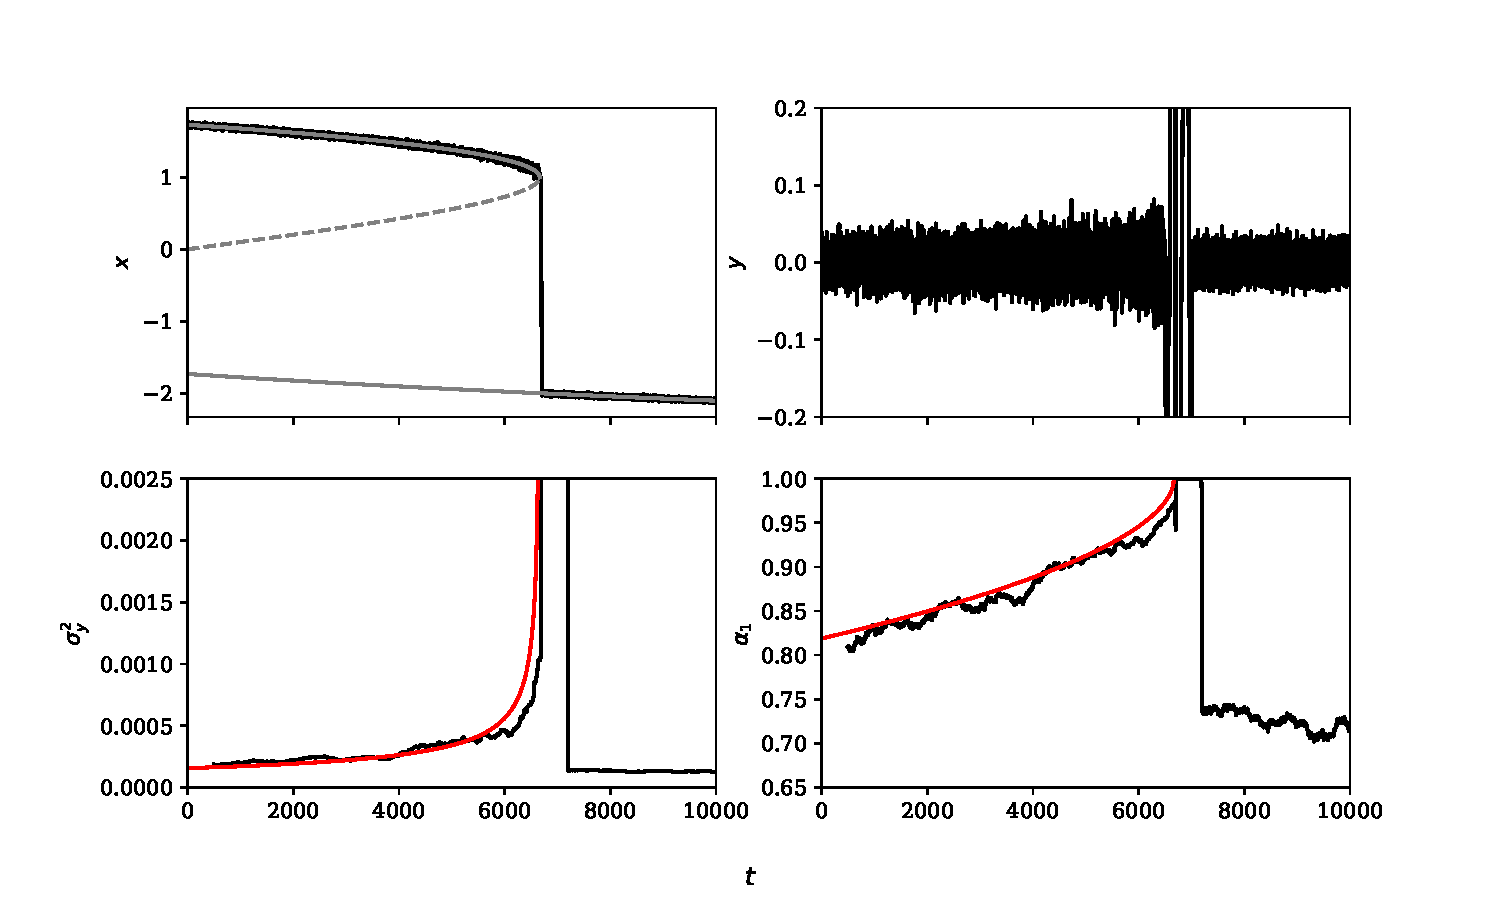
\includegraphics[width=\textwidth,keepaspectratio]{ews}
  \caption[An example of an early warning signal]{An example of using early warning signals to detect an approaching tipping point. In the top left is the original time series in black, obtained
    from integrating \cref{eq:ews_system} with a timestep of $0.1$. Also shown in grey are the quasi-static equilibria, where the unstable equilibria are shown with a dotted line.
    The top right shows the time series detrended using a cubic polynomial in windows of length 500 time units.
    The bottom left shows the variance of the detrended time series with the variance calculated through \cref{eq:y_var} in red. The bottom right shows the autocorrelation of the detrended time series
    with the autocorrelation calculated by \cref{eq:y_ac} shown in red. There is a clear early warning signal of rising variance and autocorrelation before the bifurcation.}
  \label{fig:ews}
\end{figure}

\subsection{Other Early Warning Signals}
These indicators have been generalised to higher dimensional and periodically forced systems \parencite{Williamson2015,Williamson2016}. Attempts have also been made to estimate
$\lambda$, the inverse timescale directly \parencite{Boettner2022,Boers2021a}. The idea to look at
changes in timescale of fluctuations has been investigated using Detrended Fluctuation Analysis \parencite{Livina2007}, where it was used to anticipate the warming at the
end of the Younger Dryas. Changes in these timescales can also lead to spectral reddening \parencite{Kleinen2003}. Higher order moments have proved useful too, such as the
skewness \parencite{Guttal2008} and kurtosis \parencite{Xie2019}. The phenomenon of flickering \parencite{Wang2012}, in which systems `flicker' back and forth between alternative stable
states can also be used to detect upcoming transitions. More recently, machine learning techniques have had success in giving early warning for modelled transitions \parencite{Bury2021}.
Any measure of resilience of an ecosystem can function as an early warning indicator, see~\cite{Krakovska2023} for examples of ecological resilience.


Methods which calculate the early warning statistics over space rather than over time have also been used \parencite{Donangelo2010,Guttal2009}. Changes in spatial
patterns, for example of vegetation, have also been suggested as early warning indicators \parencite{Kefi2007,Kefi2014} although introducing spatial dynamics can complicate the analysis
of tipping points \parencite{Rietkerk2021}.

Whilst these indicators generally try to be generic --- in that they are applicable to many different systems --- there is no reason why early warning indicators cannot be designed for specific systems.
\cite{Parry2022} found that the seasonal cycle in temperature was a potential early warning system for Amazon dieback and~\cite{Boulton2013} found the sensitivity of net ecosystem productivity to temperature decreases
towards the tipping point.

\subsection{The Use of Early Warning Signals}
Early Warning Signals have been applied to the Earth system. For example~\cite{Dakos2008} applied them to a variety of abrupt shifts and found that they were preceded by rises in autocorrelation,
although some of these trends could have occurred by chance. They have also been used to provide evidence for the subpolar gyre circulation destabilising prior to the
Little Ice Age \parencite{Arellano-Nava2022}. Furthermore their presence has been
used to argue that Dansgaard-Oeschger events are B-tipping \parencite{Boers2018a} and their absence has been used to argue that Dansgaard-Oeschger events are N-tipping \parencite{Ditlevsen2010}.
These contradictory findings
are related to differences in the way the ice core data is processed.

Early Warning Signals have been investigated for the Greenland ice sheet \parencite{Boers2021}. This study suggested the ice sheet was close to a tipping point.
However given the slow response of the ice sheet and
the fast change of the climate, inequality~\ref{eq:timescale_separation} is likely to be violated with the timescale of the drift to be much faster than the timescale of the dynamics.
Furthermore, the analysis is of melt rates
rather than a state variable which describes the ice sheet itself. However, the researchers could relate the observed fluctuations to a physically motivated simple nonlinear model of the ice sheet,
which would suggest the ice sheet is approaching a tipping point.

Later that year, another paper \parencite{Boers2021a}, was published suggesting the AMOC was approaching a tipping point due to increases in autocorrelation and variance.
Other work \parencite{Ditlevsen2023} went as far
as to suggest that most likely year for the AMOC to tip is 2057. Although the dynamics of the AMOC are faster than that of the ice sheets \parencite{ArmstrongMcKay2022}, it is still not clear if
inequality~\ref{eq:timescale_separation} is satisfied but early warning signals have been used in complex models to detect AMOC shut-down \parencite{Boulton2014}.
Furthermore, the analysis was not based on the AMOC strength directly but on `fingerprints' derived from sea surface temperature and salinity data.

Recent work \parencite{Boulton2022} found increases in the autocorrelation in  the Vegetation Optical Depth (a satellite measure of vegetation biomass) in the Amazon,
which is consistent with a loss of resilience in that
ecosystem. The results for changes in variance were more equivocal. Whilst the Amazon is a relatively fast tipping point \parencite{Ritchie2021}, some complex models do not show
generic early warning signals before the
tipping point \parencite{Boulton2013}. Other work \parencite{Fernandez-Martinez2023}, which examined global datasets of net biome productivity, did not find increasing autocorrelation
over the Amazon. However net biosphere productivity is a flux, not a state variable.